\chapter{Problem Analysis}
This chapter will strive to answer the research questions posed in \ref{sub:ResearchQ} and any other relevant information that arises. Additionally, a final problem will be stated after the research is complete.


\section{Research}
This section focuses on the research necessary for the basic understanding of the subject. This will include a short description of some effects that could be applied by the system, the current state of the art within the field, and some theory behind the use of gestures.

\subsection{Effects}
Many voice effects exist today. Some effects are used in most music, and some are not. The effects can be really subtle, or really noticeable.
In this section, there will be short descriptions of some common effects.


\subsubsection{Delay}

A delay effect creates a repetition of the original sound after a period of time\citep{Loeffler_2014}. By using the delay effect, it is possible to simulate the sound of the echo created when yelling into a cave or over a canyon.

\subsubsection{Reverberation}

When sound reflects off surfaces in a confined space, its called natural reverberation\citep{Redmon_1997}. Reverberation like this works best when the sound hits hard surfaces. For example, the sound effect that comes when you sing or yell in a church, is reverberation. The sound bounces all around the church's hard walls.
Digitally, the way to simulate reverberation is to use a multitude of delays and feedback. This then creates a series of echoes that then slowly decays.

\subsubsection{Pitch Shift}

The frequency of a harmonic sound is called its pitch\citep{Katjaas_00}. By shifting the pitch, the sound will effectively become deeper or higher. An example of this is the voice that anonymous people get when they want to hide their voice, this is a lowered pitch. Another example is the “chipmunk voice”, which is achieved through a raised pitch.
Pitch shifting can be done by using the "phase vocoder", which is a digital signal processing technique\citep{dolson}. The phase vocoder works by analysis and synthesis. The analysis part takes the signal, and models it as a sine wave in which one can find the amplitude, phase, and frequency of the sine wave. In the synthesis part, one can manipulate these parameters. 
The phase vocoder can do many things, e.g. change the pitch of a sound without changing the duration of the sound - make a sound deeper or higher. 

Pitch shifting is also used to create the harmonizer effect. It takes the input voice and shifts its pitch a certain amount, and then adds it as an additional voice. This can effectively simulate a choir.

\subsubsection{Auto-Tune}

The Auto-tune effect corrects a singer's voice to the correct tone\citep{Hadhazy_2010}. This can be really subtle or plainly obvious. 
The user just needs to choose a reference of scales or tones and the amount of correction that needs to be made, and then the Auto-tune will make the proper adjustments.

\subsubsection{Vocoder}

The Vocoder effect combines a singer's voice with another sound - that could be the sound from an instrument or a synthesizer\citep{Vocoder_00}. 
The effect can make the voice sound like a robot. The vocoder needs two inputs, the voice and e.g. an instrument. The fundamental frequencies of the voice are converted to levels of amplitude on a series of band pass filters, which then are passed through the instrument sound.


\subsection{State of the Art}
To gain understanding of what is possible, a study of the state of the art was conducted with the focus on commercial artefacts used for real-time alterations.

\subsubsection{TC Helicon Perform V}

The TC Helicon - Perform V is a vocal multi-effects processor that attaches to a microphone stand, as seen in figure \ref{tchelicon}\citep{TC}. It has three effect buttons, three preset buttons, a big knob, and other buttons. The effects are reverb, echo, “double” (harmonizer), equalizer, compressor, and many more. It is possible to download an application that can connect with the Perform V. The application has many pre-made sounds, and it has a wireless connection. \\

\begin{minipage}{\linewidth}% to keep image and caption on one page
\makebox[\linewidth]{%        to center the image
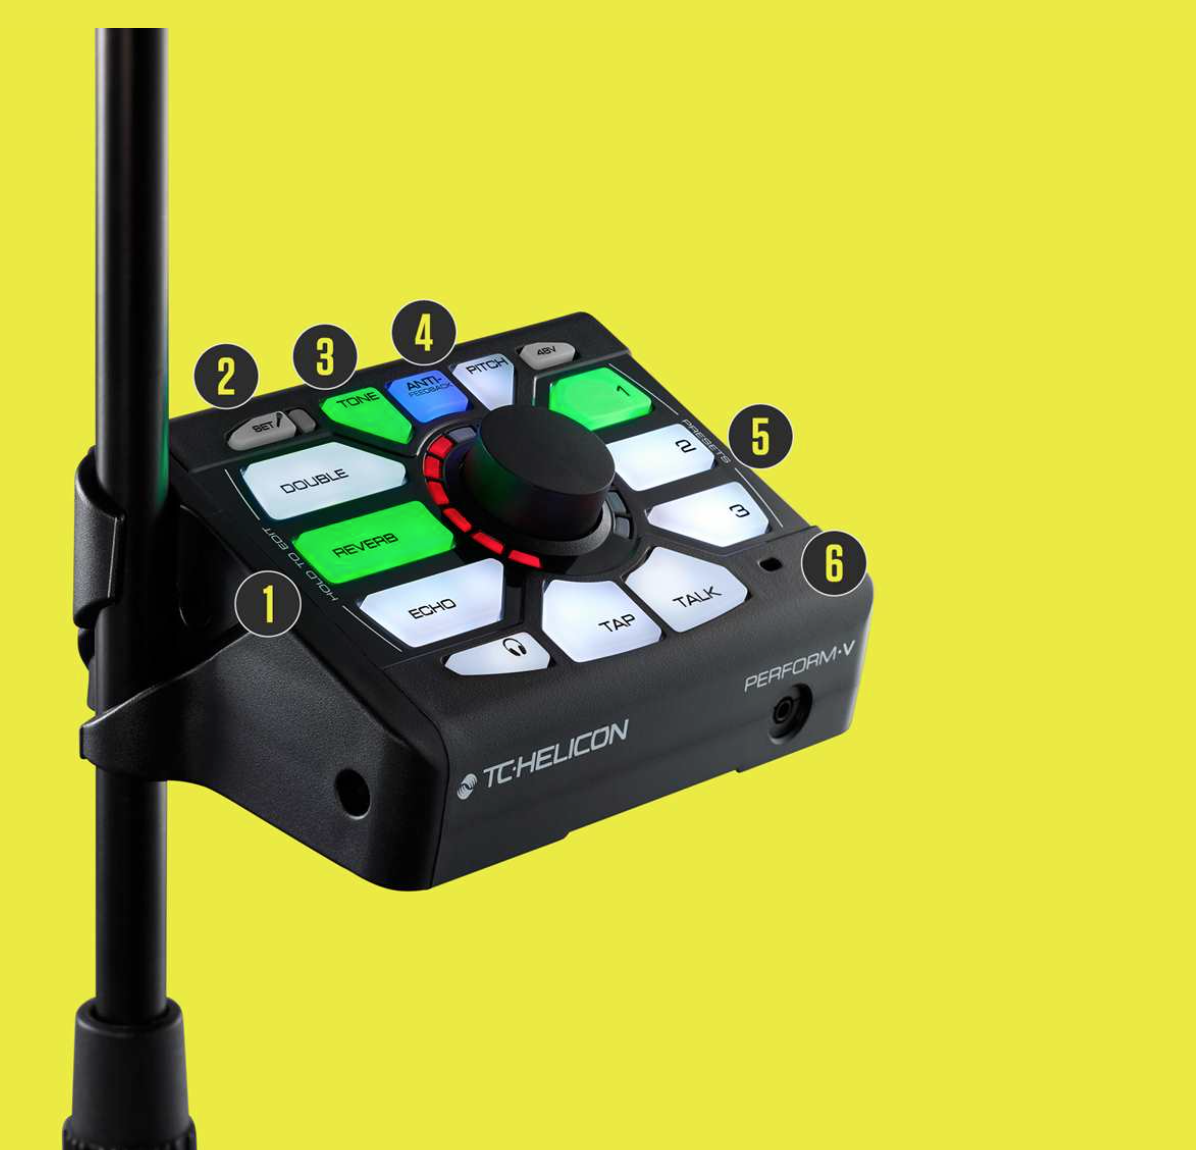
\includegraphics[keepaspectratio=true,scale=0.4]{tchelicon}}
\captionof{figure}{TC Helicon Perform V\citep{TC}}\label{tchelicon}
\end{minipage}\\

The Perform V is good for live performing if the singer has the processor in front of them, on the microphone stand. Preset buttons make it easy to change effect quickly. 
If the singer plays an instrument, it is probably difficult to change effects without interrupting the instrument playing. Another downside is that the singer is limited to only three presets, and only one knob to turn.

\subsubsection{Electro Harmonix Voice Box}

The Electro Harmonix Voice Box is a more advanced processor than the TC Helicon\citep{VoiceBox}. It has six knobs: blend, two reverb knobs, “gender bender”, voice mix, and “Mode”, as seen in figure \ref{voice_box}. It has nine different modes, which includes different kinds of harmonies, unison-whistle, and a vocoder, which the TC Helicon does not have.\\

\begin{minipage}{\linewidth}% to keep image and caption on one page
\makebox[\linewidth]{%        to center the image
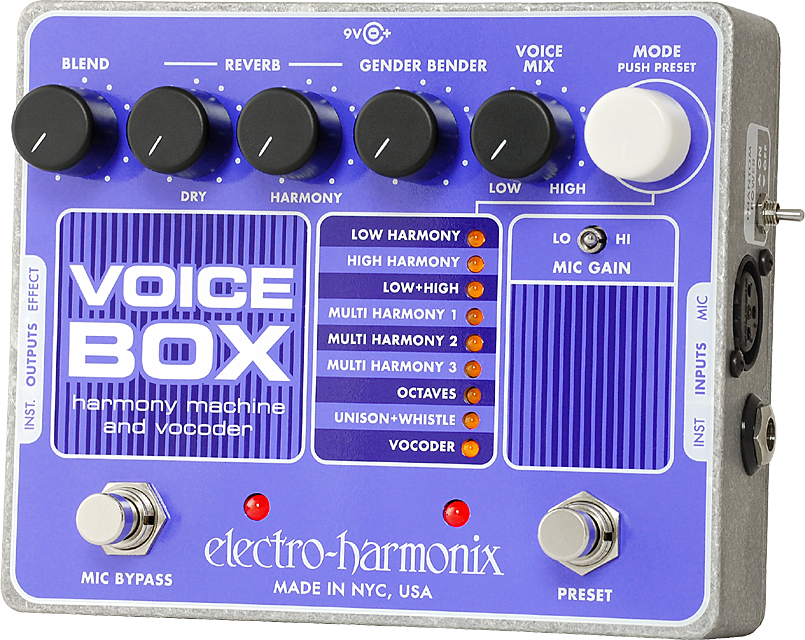
\includegraphics[keepaspectratio=true,scale=0.4]{voice_box}}
\captionof{figure}{Electro Harmonix Voice Box\citep{VoiceBox}}\label{voice_box}
\end{minipage}\\

The Voice Box has to be on a flat surface, like the floor or a table and is most often used as a pedal. It is possible to insert an instrument into the pedal, so it can be used for the vocoder. The Voice Box has many effects and knobs - this can make changing effects and effect parameters difficult, even more if the pedal is on the floor.

\subsubsection{Mi.Mu Gloves}

The Mi.Mu Gloves are gloves made for making music, and controlling sound\citep{Mimu}. They are made by scientists, musicians, and artists, and have been in development since 2010. They are wearable, and can be used by one or both hands, see figure \ref{mimu}. The gloves have been through many iterations, and they are open source. The gloves use gestures, hand and finger movement, finger placement, and other features to control sounds and effects. The hardware includes an ArduImu, flex/bend sensors, accelerometer, gyroscope, haptic motors, LED's, WiFi compatibility, and provides other capabilities.\\

\begin{minipage}{\linewidth}% to keep image and caption on one page
\makebox[\linewidth]{%        to center the image
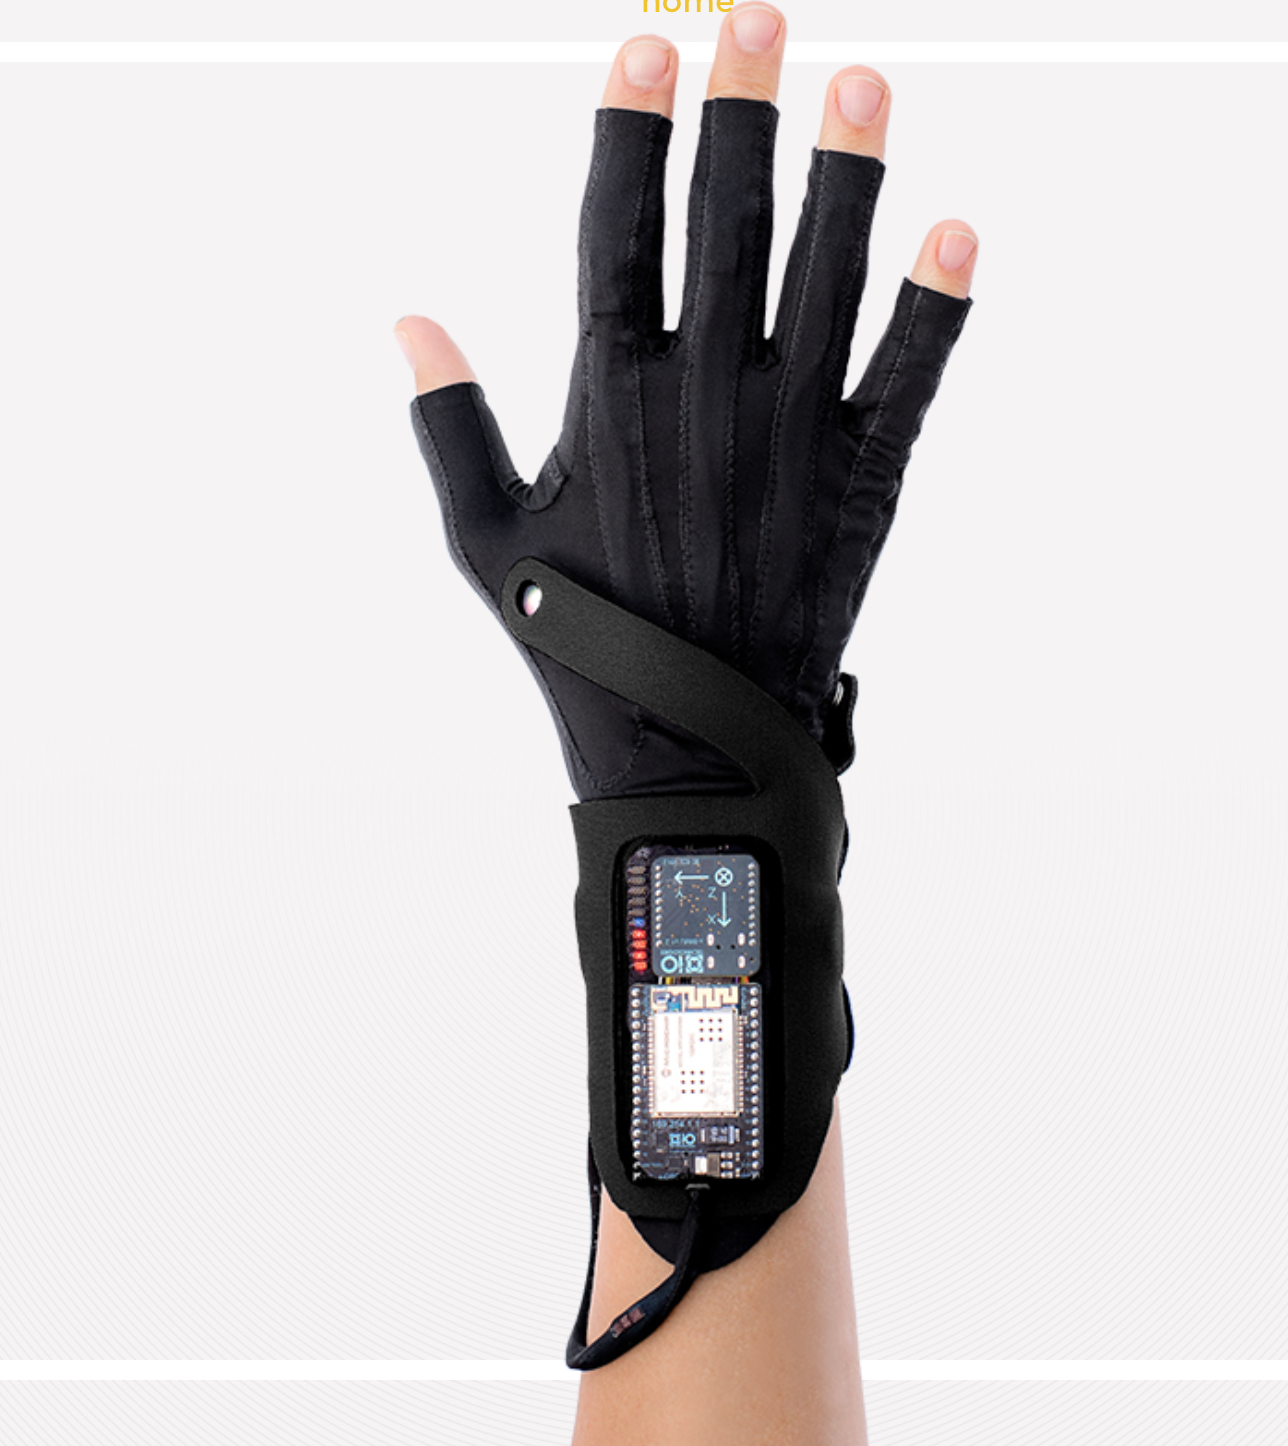
\includegraphics[keepaspectratio=true,scale=0.4]{mimu}}
\captionof{figure}{Mi.Mu Gloves\citep{Mimu}}\label{mimu}
\end{minipage}\\

The gloves are bluetooth or Wi-Fi connected, so the person using the gloves are free to move around, and does not have to worry about wires. They are also battery powered. 
Since the gloves are open source, you can make your own - many different gloves exist - some are simple, and some are complex.

\subsubsection{HandySinger: Expressive Singing Voice Morphing using Personified Hand-puppet Interface}

Yonezawa et al. made a glove that controls voice effects \citep{Yonezawa_2005}. The wearer of the glove controls a puppet and and makes hand gestures, see figure \ref{puppet1}. \\

\begin{minipage}{\linewidth}% to keep image and caption on one page
\makebox[\linewidth]{%        to center the image
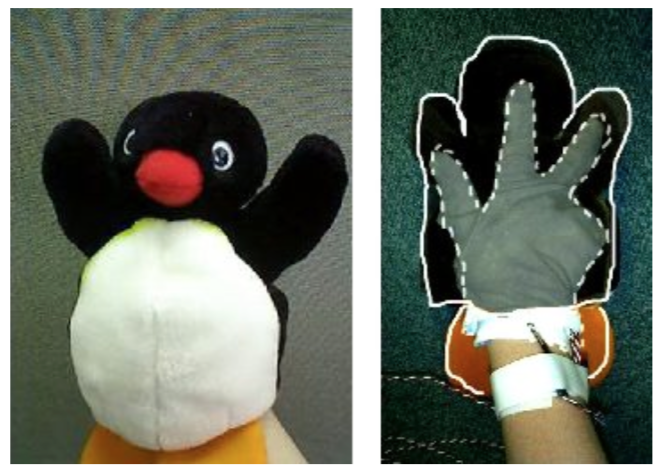
\includegraphics[keepaspectratio=true,scale=0.4]{puppet1}}
\captionof{figure}{HandySinger Glove \citep{Yonezawa_2005}}\label{puppet1}
\end{minipage}\\

They believe that using a puppet interface will increase the expressiveness of the user’s singing voice. The glove itself has seven bend sensors, and two pressure sensors, see figure \ref{puppet2}. \\

\begin{minipage}{\linewidth}% to keep image and caption on one page
\makebox[\linewidth]{%        to center the image
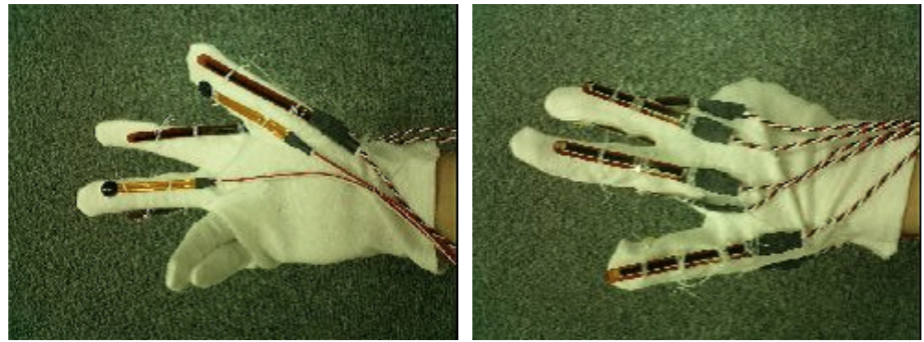
\includegraphics[keepaspectratio=true,scale=0.4]{puppet2}}
\captionof{figure}{HandySinger Glove sensors \citep{Yonezawa_2005}}\label{puppet2}
\end{minipage}\\

The glove measures both forward bend and backwards bend. The gestures that the users can make are: bend back clasp, drooping, stretching, and bend back. The parameters that the gestures change are: “dark”, “whisper”, “wet”, and volume. Yonezawa et al. found that users with small hands had trouble using the glove effectively. Nevertheless, they confirmed it was easy to gesture with the hand-puppet and that the gestures reflect the voice expression changes.

\subsubsection{The 'One-Person Choir': A Multidisciplinary Approach to the Development of an Embodied Human-Computer Interface}
The study by, Maes et al. \citep{Maes_2011} utilises body gesture to enhance a singer's voice. The system is a human-computer interface that use gestural control for harmonising a singing voice. The system is operating in real-time, which means it is possible to use it during live performances. The system uses pre-configured models to control the harmonisation, and the singer can eventually use this to enhance his or her singing voice. 
During their research, they found that gesture control is a big part of singing, which also helps the perception of the singing. The movement of the upper body is the primary gesture used in the system which means that the singer has sensors attached to the upper body.


\subsection{Gestures}

When designing a way to control effects, there are several ways to approach it. One of these ways is through gesture control.

There are also several ways to approach gesture control. For example, there are three stages of a gesture: registration, continuation, and termination\citep[pp. 127-134]{Wigdor_2011}.\\

\begin{minipage}{\linewidth}% to keep image and caption on one page
\makebox[\linewidth]{%        to center the image
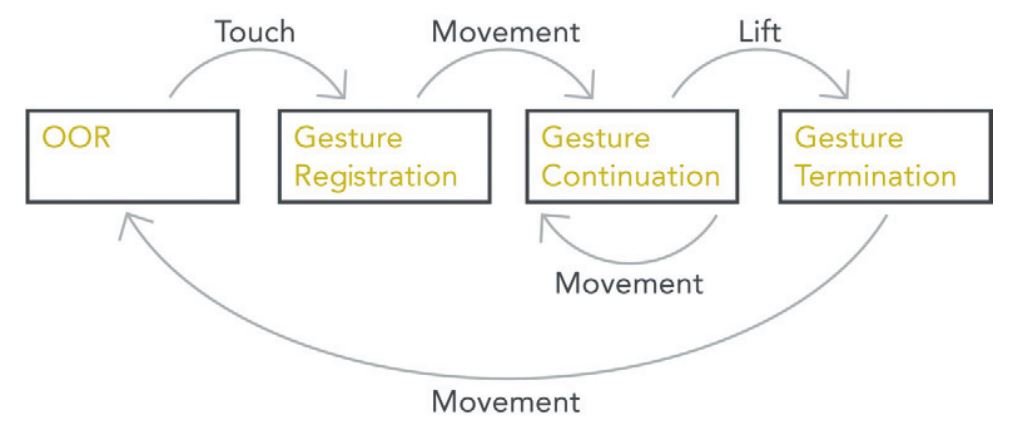
\includegraphics[keepaspectratio=true,scale=0.4]{Gestures}}
\captionof{figure}{Out of Range(OOR) and the three stages of gestural input \citep[pp. 127]{Wigdor_2011}}\label{Gestures}
\end{minipage}\\

The registration stage is when the system registers that the user would want to perform a gestural input, e.g. when you place your finger(s) on a touch display. 

The next stage is continuation. In this stage, the user uses movement to adjust the parameters of the gesture, e.g. when you move two fingers away from each other in order to zoom, on a touch display.

The final stage is termination, where the user simply ends the gesture, e.g. by lifting their finger(s) from a touch display.

In some cases the continuation stage can be skipped. Whether or not it is a good idea to skip this stage is decided by the number of different gestures one wants to implement, and whether they want the gesture to be able to change the parameters or not, e.g. a zoom that does not have one set amount of zoom, but rather it is specified by how much you move your fingers. By removing the continuation stage, it also removes the possibility to differentiate between a lot of gestures. \\

A good thing to do, when choosing a gesture for a specific action, is to keep it as unambiguous as possible. This helps reduce future errors. This being said, it is also important to minimise the amount of steps the user has to go through for the gesture.

While the previously mentioned ‘zoom’ gesture is a rather good example of a gesture, a bad example of a gesture would be the use of the ‘flick’ action to execute a gesture. The ‘flick’ action is when you execute an action by ‘flicking’ an object to e.g. delete it. The bad thing about this design is the fact that you have to specify a border between the action of moving something and ‘flicking’ something


\subsection{Conclusion}




\section{Problem Statement}
From the research a final problem statement has been made, and it sounds:\\

\textit{Audio effects for the voice exist but they are impractical to change while performing. Technology exists that address this problem, e.g. gloves that use sensors. We want to make a glove that can change voice effect and their parameters.}

\subsubsection{Success Criteria}

\begin{itemize}
	\item The system should have at least two effects
	\item Users use the right gestures to change the effects
	\item The system does the right action to the gesture - does not misinterpret 
\end{itemize}



\section{Minimum Implementation}
\begin{itemize}
	\item The design must implement the use of an Arduino
	\item The design must implement the use of sensors applicable to the Arduino
	\item The design must implement audio processing
	\item The design must get audio from a microphone
\end{itemize}

